\documentclass[11pt]{article}
\usepackage[margin=1in]{geometry}
\usepackage{amsmath,amssymb,amsthm}
\usepackage{graphicx}
\graphicspath{{../figures/}}
\usepackage{xcolor}
\usepackage{booktabs}
\usepackage[numbers,sort&compress]{natbib}
\usepackage{xurl}
\usepackage[colorlinks=true,linkcolor=blue!50!black,citecolor=blue!50!black,urlcolor=blue!50!black]{hyperref}

\newtheorem{theorem}{Theorem}
\newtheorem{lemma}{Lemma}
\newtheorem{corollary}{Corollary}
\theoremstyle{remark}
\newtheorem{remark}{Remark}

\newcommand{\Hhat}{\hat{H}}
\newcommand{\Vhat}{\hat{V}}
\newcommand{\dd}{\mathrm{d}}
\newcommand{\Ind}[1]{[\,#1\,]}


\title{Stability of a negative-mass boson star}
\author{Nathan Moinvaziri\thanks{\href{mailto:nathan@nathanm.com}{nathan@nathanm.com}}\\[2pt]
\normalsize\textit{Independent researcher}}
\date{October 2026}

\begin{document}
\maketitle

\begin{abstract}
A complex scalar whose stress tensor enters Einstein's equations with a minus sign forms stationary, regular stars of
negative ADM mass; such a star was recently used as the negative partner in full numerical-relativity simulations of
Bondi's runaway pair. We give its first linear stability analysis. Radially, the configuration used in those simulations
is stable, and the family loses stability exactly where the Noether charge $N$ is extremal. Because the first law
becomes $\dd M=-\omega\,\dd N$, the turning-point criterion holds in $N$ but reverses sign when written in $M$.
Spherically symmetric nonlinear evolutions confirm the stationarity of stable stars to $t=1500$ and the predicted growth
rates of unstable ones, and show that slow drifts reported in $3+1$ are not a property of the spherical dynamics.
Non-radially, we derive the polar and axial perturbation equations with the sign of the coupling kept symbolic and find
no unstable $\ell=2,3$ polar mode and no unstable axial mode, in ranges that contain the growth rates of the
negative-mass Schwarzschild instability. The effective surface condition the star supplies to its vacuum exterior lies
above the critical value of a companion paper, so the point-mass instability is not triggered.
\end{abstract}

\tableofcontents

\section{Introduction}

Bondi's 1957 analysis~\cite{Bondi1957} showed that general relativity contains no logical obstruction to negative
mass, provided inertial, passive and active mass share a sign, and that a pair of equal and opposite masses
self-accelerates. Recent full $3+1$ evolutions~\cite{Shirokov2026} realise the pair with a canonical boson star and a
``phantom'' boson star of negative ADM mass. Whether the phantom star is itself stable has not been examined.

Two instabilities could threaten it. The vacuum exterior is negative-mass Schwarzschild, which has one growing
even-parity mode per multipole~\cite{GD2006,DG2009}. A companion paper~\cite{Moinvaziri2026a} shows that this mode lives on a
shell of radius $\approx10|M|/\ell^2$: for the exterior of a star of radius $R$ with an interface condition
$\hat\Psi'=\kappa\hat\Psi$ on the Dotti--Gleiser variable, the number of unstable modes is
$[R<r_s]+[\kappa<\kappa_c(R)]$, with $r_s=6|M|/[(\ell+2)(\ell-1)]$ and $\kappa_c=\partial_x\ln\phi_0$ in closed form,
$\phi_0=1/\psi_0$ the static Dotti--Gleiser solution. For large $R$, $\kappa_c\approx-(\ell+1)/R$; for $\ell=2$ every
$\kappa\ge0$ is stable once $|M|/R<0.439$. The second threat is the matter itself, through the radial turning-point
instability familiar from ordinary boson stars~\cite{GW1989,LeePang1989,KMS1991} or through non-radial modes.

We address both. Section~\ref{sec:model} sets up the model; Sec.~\ref{sec:radial} gives the radial analysis and
Sec.~\ref{sec:evol} nonlinear evolutions; Sec.~\ref{sec:nonradial} the non-radial analysis, including the surface
condition $\kappa_{\rm eff}$ the star supplies. Units $G=c=1$ and scalar mass $m=1$. All computations are reproducible from
\url{https://github.com/nmoinvaz/negative-mass}.

\section{Model and static stars}\label{sec:model}

\paragraph{Model.} Following Ref.~\cite{Shirokov2026}, take a complex scalar with
$\mathcal L=-\tfrac12|\nabla\Phi|^2-V(|\Phi|^2)$, $V(s)=\tfrac12s-\tfrac14\lambda s^2+\tfrac16\mu s^3$, $\lambda=10240$,
$\lambda^2/\mu=4.8$, coupled through
\begin{equation}
G_{ab}=8\pi\varepsilon\,T_{ab}[\Phi],\qquad \Box\Phi=2V'(|\Phi|^2)\Phi,
\end{equation}
with $\varepsilon=+1$ (canonical) or $\varepsilon=-1$. For $\varepsilon=-1$ the field equation is unchanged but the
star gravitates with negative ADM mass. In the language of Bondi, the scalar has a single mass parameter that is
inertial, passive and active at once, and is negative for $\varepsilon=-1$; gravity alone cannot distinguish this from
Bondi's ``all three negative''~\cite{Bondi1957,Bonnor1989}. The action is that of a ghost, so the model is a classical
probe; quantum mechanically it is unstable to vacuum decay~\cite{CJM2004}.

\paragraph{Static stars.} Stationary solutions $\Phi=\phi(r)e^{-i\omega t}$ in Schwarzschild-like coordinates are
solved as two-point boundary-value problems with a decaying Yukawa tail. The configuration of Ref.~\cite{Shirokov2026}
at $\omega=0.7603$ has $M=-0.014580$, rms radius $4.40$ and $|M|/R\approx3\times10^{-3}$, far below the threshold
$|M|/R<0.439$ of Ref.~\cite{Moinvaziri2026a}: the shell where negative-mass Schwarzschild would be unstable lies deep inside the
matter. (Our masses are ADM masses; those quoted in Ref.~\cite{Shirokov2026} are the mass enclosed where $\phi$ falls to
$5\%$ of its central value and are $1.5$--$2.3\%$ smaller; the field profiles agree to $10^{-5}$.)

\paragraph{First law.} With $N=\int4\pi r^2\omega\phi^2(a/\alpha)\,\dd r$ the Noether charge, the family satisfies
\begin{equation}
\dd M=\varepsilon\,\omega\,\dd N,
\end{equation}
verified by finite differences to $<10^{-4}$. Hence $M(\omega)$ and $N(\omega)$ are extremal at the same $\omega$ for
either sign, but $\dd M/\dd\omega$ and $\dd N/\dd\omega$ have opposite signs when $\varepsilon=-1$.

\section{Radial stability}\label{sec:radial}

\paragraph{Radial perturbations.} Perturbing the metric functions and both components of the field with
$e^{i\sigma t}$, we eliminate the metric through the $tr$ and $rr$ constraints and obtain a closed fourth-order system for
the real perturbation, a gauge-invariant phase and the perturbed enclosed charge, containing $\sigma$ only as $\sigma^2$
and $\varepsilon$ symbolically. Substituting back, all six linearised field equations are satisfied identically. The
structure is that of Refs.~\cite{GW1989,Kain2021}. Eigenvalues are found by compound-matrix shooting, which keeps the
two-dimensional space of decaying solutions well conditioned, and are cross-checked by an independent finite-difference
pencil that also returns complex eigenvalues.

\begin{figure}[t]
\centering
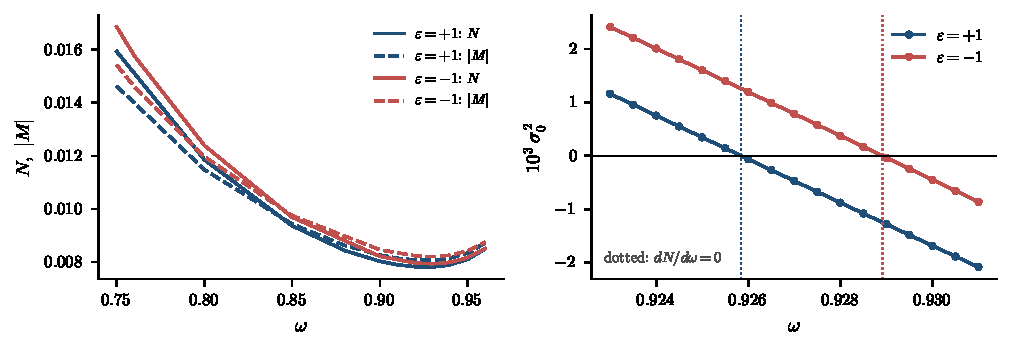
\includegraphics[width=0.97\textwidth]{fig4_radial.pdf}
\caption{Radial stability of signed-source boson stars. Left: Noether charge $N$ and $|M|$ along the canonical
($\varepsilon=+1$) and phantom ($\varepsilon=-1$) families. Right: fundamental $\sigma_0^2$ near the stability change;
dotted lines mark $\dd N/\dd\omega=0$, which coincides with $\sigma_0^2=0$ to $2\times10^{-8}$ ($\varepsilon=+1$) and
$8\times10^{-8}$ ($\varepsilon=-1$) in $\omega$.}
\label{fig:radial}
\end{figure}

\paragraph{Results.} For $\varepsilon=+1$ the textbook criterion is reproduced at both turning points of the family: the
fundamental mode crosses zero at $\omega=0.92584444$ against $\dd M/\dd\omega=\dd N/\dd\omega=0$ at $0.92584446$, and
again at the strong-field maximum of $N$ ($\omega\approx0.200$, $N\approx42.73$) within the scan resolution. For
$\varepsilon=-1$ (Fig.~\ref{fig:radial}):
\begin{itemize}
\item The star of Ref.~\cite{Shirokov2026} is radially stable: no real growth rate up to $|\sigma|=2$ and no complex
eigenvalue with $|\sigma^2|<0.3$, at two resolutions of the finite-difference check.
\item The family is stable for $\omega<0.92891$ and unstable above. The crossing $\sigma_0^2=0$ at $\omega=0.92890846$
coincides with $\dd N/\dd\omega=0$ at $0.92890838$.
\item The criterion is therefore invariant when stated in $N$ (stable side $\dd N/\dd\omega<0$) but reverses when
stated in $M$: on the stable side $\dd M/\dd\omega=-\omega\,\dd N/\dd\omega>0$.
\item The phantom family has a fold in $\omega$ ($\omega_{\min}\approx0.4223$) at which neither $M$ nor $N$ is
extremal; the fundamental mode stays positive through it. The strong-field branch, followed to $|2m/r|\approx0.4$, is
stable with no turning point.
\end{itemize}
Near $\omega\approx0.93$ the instability is essentially the flat-space Vakhitov--Kolokolov instability of
$Q$-balls~\cite{Coleman1985,FLP1987}, with gravity a small correction; the strong-field branch is the more sensitive
test of how $\varepsilon$ enters. The first law and the $N$-form of the criterion follow from the standard turning-point
arguments~\cite{Sorkin1982,LeePang1989,KMS1991} with $\varepsilon$ kept; the new content is the explicit linear analysis
for $\varepsilon=-1$. The result is consistent with the theorem that barotropic negative-mass stars are radially
unstable~\cite{Alves2025}, which does not apply to scalar-field matter.

\section{Nonlinear evolution}\label{sec:evol}

We evolve single stars in spherical symmetry in polar-areal slicing, re-solving the
Hamiltonian constraint for the Misner--Sharp mass~\cite{MisnerSharp} and the slicing condition at every substep, with
$\varepsilon$ appearing only there~\cite{SeidelSuen1990,HawleyChoptuik2000}. The scheme is fourth order in space and time
and converges at order $\approx4$; the Misner--Sharp mass outside the star equals the ADM mass of the static solution to
$5\times10^{-8}$. Unstable stars at $\omega=0.94$, perturbed by $\pm\delta$, grow at $\sigma=0.07376$ ($\varepsilon=+1$)
and $0.06679$ ($\varepsilon=-1$) against $0.07370$ and $0.06668$ from the linear analysis (Fig.~\ref{fig:evol}, right).
The stable campaign stars of both signs remain stationary to $t=1500$, with fractional drifts of $\omega$, the central
amplitude, the Misner--Sharp mass and $N$ all $\le10^{-6}$ at $h=0.1$ and decreasing with resolution
(Fig.~\ref{fig:evol}, left). A $5\%$ perturbation relaxes within $\sim150$ time units onto the neighbouring static star
and stays there. The slow drifts reported for a lone phantom star in $3+1$~\cite{Shirokov2026} are therefore not a
property of the spherical dynamics.

\begin{figure}[t]
\centering
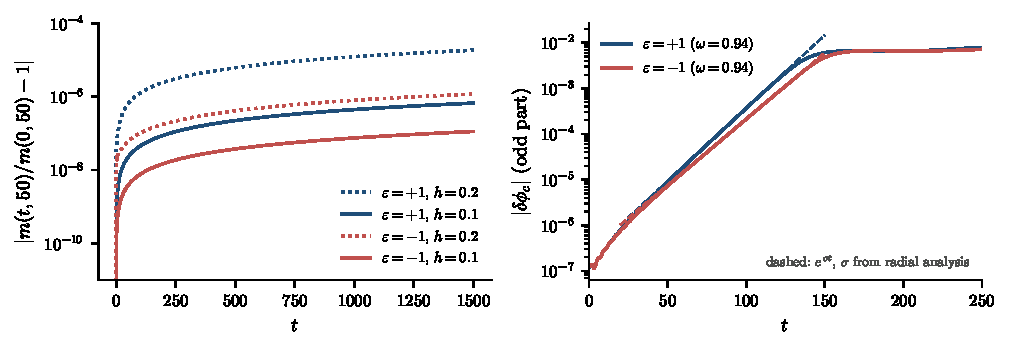
\includegraphics[width=0.97\textwidth]{fig5_evolution.pdf}
\caption{Spherically symmetric nonlinear evolutions. Left: relative drift of the Misner--Sharp mass at $r=50$ for the
stable campaign stars ($\omega=0.750$ canonical, $\omega=0.7603$ phantom) at two resolutions; the drift is a
dissipation-limited truncation error that decreases rapidly with $h$. Right: odd part of the central-amplitude response
of unstable stars ($\omega=0.94$) to $\pm10^{-5}$ perturbations; dashed lines have the growth rates of the linear
analysis.}
\label{fig:evol}
\end{figure}

\section{Non-radial stability}\label{sec:nonradial}

For $\ell\ge2$ we linearise in Regge--Wheeler gauge with $\varepsilon$ symbolic.
In the polar sector the traceless angular equation gives $H_2=H_0$, and the $(rr)$ equation must be solved jointly with
both Klein--Gordon equations; the result is a sixth-order system for
$y=(H_1/s,\,K,\,F,\,F',\,G/s,\,G'/s)$, polynomial and even in
$s$, generated by computer algebra. All eight separated field equations hold on its solutions to $7\times10^{-7}$; in
vacuum it reduces exactly, through the Moncrief map, to the Zerilli equation plus a free scalar; and for $\varepsilon=+1$
it reproduces the fundamental $\ell=2$ polar mode of a published mini boson star~\cite{Macedo2013},
$\sigma=0.119519-5.35\times10^{-5}i$. The axial sector reduces to
\begin{equation}
Q_{,r_*r_*}=(s^2+V_{\rm ax})Q,\qquad V_{\rm ax}=e^{\nu}\big[\ell(\ell+1)/r^2-6m/r^3+8\pi\varepsilon V(\phi_0^2)\big].
\end{equation}

Growing modes are sought with a matching determinant between the three regular interior solutions and the decaying
exterior (Zerilli plus Yukawa) solutions, integrated with continuous orthonormalisation. For the phantom star the
determinant has no real zero for $\gamma\in[10^{-3},300]$ ($\ell=2$) and $[10^{-3},1000]$ ($\ell=3$), ranges that contain
the point-mass rates $137$ and $686$; the same holds for phantom stars at $\omega=0.70$ and $0.85$ and for the canonical
star. An argument-principle count, validated on the known mode above, finds no zero with $0.1\le\Re s\le2$,
$|\Im s|\le2.5$, which also excludes oscillatory matter-sector instabilities in that region. The axial potential is
positive for every $\ell\ge2$ and every star examined, so the axial sector is stable.

The interior acts on the exterior through $\kappa_{\rm eff}(\ell,s)$, and the intertwiner gives the exact relation
$\kappa_{\rm eff}-\kappa_c=s^2/(q_{\rm int}-g)$, with $q_{\rm int}$ the interior log-derivative and $g=\partial_x\ln\psi_0$.
Hence $\kappa_{\rm eff}\to\kappa_c$ as $s\to0$ for any star, with the sign fixed by a static tidal (Love-type)
coefficient. For the phantom star, $\kappa_{\rm eff}>\kappa_c$ at every $\gamma$ tabulated in $[10^{-4},150]$; it becomes
positive at $\gamma\approx2\times10^{-4}$ and then grows like $\gamma|M|$. By the count of Ref.~\cite{Moinvaziri2026a} the star never
supplies the $\kappa<\kappa_c\approx-(\ell+1)/R$ an instability would need. These are scans, not proofs: a closely spaced
pair of real roots, slowly growing modes with $\Re s<0.1$, and $\ell\ge4$ are not excluded.

\section{Discussion}\label{sec:discussion}

The phantom boson star of Ref.~\cite{Shirokov2026}, which is dilute ($|M|/R\sim10^{-3}$), is radially stable, shows
no unstable $\ell=2,3$ polar or axial mode, and supplies $\kappa_{\rm eff}>\kappa_c$, so the vacuum instability of
negative-mass Schwarzschild is not triggered. The radial criterion is the familiar one once stated in the Noether charge,
and reverses sign when stated in the mass. Extending the non-radial scans to higher $\ell$, to slowly growing modes, and
to compact phantom stars, where $|M|/R$ approaches the thresholds of Ref.~\cite{Moinvaziri2026a}, is the natural next
step.

The results are classical: the phantom sector is a ghost, and a quantum theory of it has an unstable
vacuum~\cite{CJM2004}.

\section{How the results were obtained}\label{sec:method}

The author set the questions and scope and reviewed each stage; Anthropic's Claude, run as an agent with a Python
environment and parallel sub-agents, did the literature reading, derivations, code and drafting. No claim rests on
the assistant's word alone:
\begin{itemize}
\item \emph{Starting points.} The stars of Ref.~\cite{Shirokov2026} were reproduced to $10^{-5}$ in the field profile,
and the $2\%$ mass offset traced to the definition of mass used there.
\item \emph{Equations.} Perturbation equations were generated by computer algebra with $\varepsilon$ symbolic and checked
against every linearised field equation, the vacuum (Zerilli) limit and a published quasinormal mode.
\item \emph{Numerics.} Each radial eigenvalue was computed by two independent methods; the evolution code was checked by
convergence order, mass conservation and recovery of the linear growth rates.
\item \emph{Review.} Separate agents audited the codes without seeing our conclusions, and a literature search preceded
every novelty claim.
\end{itemize}
These checks are internal; the work has not yet been reviewed by specialists.

\paragraph{Reproducibility.} The background, radial and non-radial perturbation codes, the nonlinear evolution code and
the figure script are in the accompanying
repository,
\url{https://github.com/nmoinvaz/negative-mass}.

\paragraph{Acknowledgments.} The author thanks Anthropic's Claude, which carried out the analysis, computations and
drafting described in Sec.~\ref{sec:method} under the author's direction.

\begin{thebibliography}{99}

\bibitem{Bondi1957} H. Bondi, ``Negative mass in general relativity,'' Rev. Mod. Phys. \textbf{29}, 423 (1957).
\bibitem{Shirokov2026} N. M. Shirokov, ``The Bondi dipole in full numerical relativity: a self-accelerating
positive--negative mass binary,'' arXiv:2608.24577.
\bibitem{GD2006} R. J. Gleiser and G. Dotti, ``Instability of the negative mass Schwarzschild naked singularity,''
Class. Quantum Grav. \textbf{23}, 5063 (2006), arXiv:gr-qc/0604021.
\bibitem{DG2009} G. Dotti and R. J. Gleiser, ``The initial value problem for linearized gravitational perturbations of
the Schwarzschild naked singularity,'' Class. Quantum Grav. \textbf{26}, 215002 (2009), arXiv:0809.3615.
\bibitem{Moinvaziri2026a} N. Moinvaziri, ``The instability of negative-mass Schwarzschild is a point-mass effect: exact thresholds for finite stars,'' companion paper (2026).
\bibitem{GW1989} M. Gleiser and R. Watkins, ``Gravitational stability of scalar matter,'' Nucl. Phys. B \textbf{319},
733 (1989).
\bibitem{LeePang1989} T. D. Lee and Y. Pang, ``Stability of mini-boson stars,'' Nucl. Phys. B \textbf{315}, 477 (1989).
\bibitem{KMS1991} F. V. Kusmartsev, E. W. Mielke and F. E. Schunck, ``Gravitational stability of boson stars,'' Phys.
Rev. D \textbf{43}, 3895 (1991).
\bibitem{Bonnor1989} W. B. Bonnor, ``Negative mass in general relativity,'' Gen. Relativ. Gravit. \textbf{21}, 1143 (1989).
\bibitem{CJM2004} J. M. Cline, S. Jeon and G. D. Moore, ``The phantom menaced: constraints on low-energy effective
ghosts,'' Phys. Rev. D \textbf{70}, 043543 (2004), arXiv:hep-ph/0311312.
\bibitem{Kain2021} B. Kain, ``Radial oscillations and stability of multiple-field boson stars,'' Phys. Rev. D
\textbf{103}, 123003 (2021).
\bibitem{Coleman1985} S. Coleman, ``Q-balls,'' Nucl. Phys. B \textbf{262}, 263 (1985).
\bibitem{FLP1987} R. Friedberg, T. D. Lee and Y. Pang, ``Mini-soliton stars,'' Phys. Rev. D \textbf{35}, 3640 (1987).
\bibitem{Sorkin1982} R. D. Sorkin, ``A stability criterion for many-parameter equilibrium families,'' Astrophys. J.
\textbf{257}, 847 (1982).
\bibitem{Alves2025} M. de Aguiar Alves, A. G. S. Landulfo and B. Arderucio Costa, arXiv:2408.00154; Phys. Rev. D
\textbf{111}, 044027 (2025).
\bibitem{MisnerSharp} C. W. Misner and D. H. Sharp, ``Relativistic equations for adiabatic, spherically symmetric
gravitational collapse,'' Phys. Rev. \textbf{136}, B571 (1964).
\bibitem{SeidelSuen1990} E. Seidel and W.-M. Suen, ``Dynamical evolution of boson stars: perturbing the ground state,''
Phys. Rev. D \textbf{42}, 384 (1990).
\bibitem{HawleyChoptuik2000} S. H. Hawley and M. W. Choptuik, ``Boson stars driven to the brink of black hole
formation,'' Phys. Rev. D \textbf{62}, 104024 (2000).
\bibitem{Macedo2013} C. F. B. Macedo, P. Pani, V. Cardoso and L. C. B. Crispino, ``Astrophysical signatures of boson
stars: quasinormal modes and inspiral resonances,'' Phys. Rev. D \textbf{88}, 064046 (2013), arXiv:1307.4812.

\end{thebibliography}

\end{document}
